\documentclass[12pt,a4paper,titlepage,oneside]{book}
\usepackage[utf8]{inputenc}
\usepackage[russian]{babel}
\usepackage[OT1]{fontenc}
\usepackage{amsmath}
\usepackage{amsthm}
\usepackage{mathrsfs}
\usepackage{indentfirst}
\usepackage{amsfonts}
\usepackage{bbold}
\usepackage[hidelinks]{hyperref}
\usepackage{amssymb}
\usepackage[left=2cm,right=2cm,top=2cm,bottom=2cm]{geometry}
%\usepackage{ dsfont }
\usepackage{ upgreek }
\usepackage[normalem]{ulem}


\usepackage{graphicx}  % Для вставки рисунков
\setlength\fboxsep{3pt} % Отступ рамки \fbox{} от рисунка
\setlength\fboxrule{1pt} % Толщина линий рамки \fbox{}
\usepackage{wrapfig} % Обтекание рисунков и таблиц текстом
\usepackage{caption}

\title{Моделирование}

%%% COMMANDS
\newcommand{\overbar}[1]{\mkern 1.5mu\overline{\mkern-1.5mu#1\mkern-1.5mu}\mkern 1.5mu}
\newcommand{\argmax}{\operatornamewithlimits{argmax}}
\newcommand{\argmin}{\operatornamewithlimits{argmin}}

%%% THEOREMS
\newtheoremstyle{break}{3pt}{3pt}{\itshape}{}{\bfseries}{.}{\newline}{}

\theoremstyle{definition}
\newtheorem{definition}{Определение}[chapter]

\theoremstyle{plain}
\newtheorem{theorem}{Теорема}[chapter]

\theoremstyle{remark}
\newtheorem{remark}{Замечание}[chapter]

\theoremstyle{remark}
\newtheorem{example}{Пример}

\theoremstyle{plain}
\newtheorem{lemma}{Лемма}[chapter]

\theoremstyle{plain}
\newtheorem{corollary}{Следствие}[chapter]

%%% MISC
\setcounter{tocdepth}{1}
\def\labelitemi{--}
\renewcommand{\qedsymbol}{\rule{0.7em}{0.7em}}
\sloppy
\binoppenalty=\maxdimen
\relpenalty=\maxdimen

%%% DOCUMENT
\begin{document}

%%% TITLE PAGE
\begin{titlepage}
\begin{center}

\vfill

Санкт-Петербургский государственный университет\\
\ \\

\vfill

{\large\bf Моделирование социально-экономических систем\\}
\ \\
Лекции 
\vfill

\hfill\vbox
{
\hbox{Доцент кафедры математического моделирования}
\hbox{энергетических систем, кандидат физ.-мат. наук}
\hbox{Александр Юрьевич Крылатов}
}

\vfill

Санкт-Петербург, 2016
\end{center}
\end{titlepage}


\tableofcontents

\chapter{Балансовая модель производства}

\section{Модель <<затрата - выпуск>> (англ. input - output)}

Предположим следующее:
\begin{enumerate}

\item[1)]Количество продукции характеризуется одним числом (у каждого экономического объекта).
\item[2)]Комплектность потребления: для выпуска продукции экономический объект должен получить продукты от других объектов.
\item[3)]Линейность : для увеличения количества производства в $n$ раз, необходимо увеличить ресурс в $n$ раз.
\item[4)]Делимость на конечный продукт и на продукт, который будет использоваться в производстве.

\end{enumerate}

$\\ $

Пусть $n$ --- количество субъектов (экономических субъектов),

$x_i$ --- количество производства продукта $i$,

$\\ $

$x$ = $\left[\begin{array}{crl}
x_1\\ x_2\\ ... \\ x_n
\end{array}\right]$,

$\\ $

$x_{ji}$ --- количество продукта j, необходимого для производства i.

$\\ $

$\begin{cases}
x_{1i} = \alpha_{1i} x_i \\
x_{2i} = \alpha_{2i} x_i \\
... \\
x_{ni} = \alpha_{ni} x_i
\end{cases}$

$\\ $

$A=\left[\begin{array}{crl}
\alpha_{11} & ... & \alpha_{1n} \\
... & ... & ...\\
\alpha_{n1} & ... & \alpha_{nn}
\end{array}\right]$

$\\ $

\begin{definition}
$A$ --- матрица коэффициентов прямых затрат (матрица технологических коэффициентов).


Матрица $A$ --- положительно полуопределённая ($z^T A z   \geq 0$, для любых ненулевых векторов $z$).
\end{definition}

$y_i$ -- количество $i$-го продукта на продажу.
$$\sum \limits_{i = 1}^{n} \alpha_{ji}x_i + y_i = x_j \qquad \forall j = \overline{1,n};$$
$$Ax+y=x \leftrightarrow y=(E - A) x$$
$$x=(E-A)^{-1}y$$
$$x_j \geq 0 \qquad \forall  j = \overline{1,n}.$$
Для того, чтобы это уравнение имело единственное решение необходимо и достаточно, чтобы  $det(E-A) \neq 0$.\\

\begin{remark}
Далее под обозначением $x \geq 0$ будем понимать покомпонентную неотрицательность вектора $x$.
\end{remark}
\begin{definition}
Квадратная матрица $A$, такая, что $A_{ij} \geq 0 \: \forall i j$, называется продуктивной, если существует хотя бы один такой вектор $\bar{x} > 0$, что $(E-A)\bar{x} > 0$.
\end{definition}
\begin{theorem}(О существовании и единственности решение балансовой системы уравнений)\label{t1.1}
Матрица $A$ продуктивна, тогда и только тогда, когда существует, единственно и неотрицательно решение системы $(E-A)x=y$ для любого  вектора $y \geq 0$.
\end{theorem}
\begin{proof}
\textit{Достаточность.}

Рассмотрим $\bar{y} > 0$ и $\bar{x} \geq 0$. $(E-A)\bar{x} = \bar{y} > 0 \quad \rightarrow \quad \bar{x} > A\bar{x} \quad \rightarrow \quad \bar{x} \geq 0$. $(E-A)\bar{x} > 0$ 
\begin{lemma}\label{l1.1}
Если $A$ -- продуктивна, то
$$\lim_{\nu \to \infty} A^{\nu} = 0 \qquad \nu \in N$$

\end{lemma}
\begin{proof}
$ \bar{x} \overset{\mathrm{def}}{>} A \bar{x} \geq 0$. Существует $\lambda : 0 < \lambda < 1$ такая, что $$\lambda \bar{x} > A\bar{x}.$$ 
Домножим обе части на $A$:
$$\lambda A \bar{x} \geq A^2 \bar{x} \geq 0$$
А теперь на $\lambda$:
$$ \lambda^2 \bar{x} > \lambda A \bar{x} \geq 0$$
Не трудно увидеть, что $\lambda^2 \bar{x} > A^2 \bar{x} \geq 0$. Тогда продолжая этот процесс получим 
$$\lambda^{\nu} \bar{x} > A^{\nu} \bar{x} \geq 0.$$
Так как $\lambda^{\nu} \to 0$ при $ \nu \to \infty$, то $A^{\nu} \to 0 $ при $ \nu \to \infty.$
\end{proof}

\begin{lemma}\label{l1.2}
Если $A$ -- продуктивна и существует такой вектор $\bar{x}$, что выполняется $\bar{x} \geq A\bar{x}$, то $\bar{x} \geq 0.$
\end{lemma}
\begin{proof}

$$\bar{x} \geq A\bar{x} \geq A^2\bar{x} \geq \dots \geq A^{\nu} \bar{x}$$
$$\bar{x} \geq A^{\nu} \bar{x} \to 0 \text{, при } \nu \to \infty$$
$$\bar{x} \geq 0$$
\end{proof}

\begin{lemma}\label{l1.3}
Если $A$ -- продуктивна, то $det(E-A) \neq 0.$
\end{lemma}
\begin{proof}
\textit{От противного.}\\
Если $A$ -- продуктивна, но $det(E-A) = 0.$\\
Пусть существует такой вектор $\hat{x} \neq 0$, и пусть $(E-A)\hat{x} = 0 \quad \overset{\mathrm{Lemma 1.2}}{\Longrightarrow} \quad \hat{x} \geq 0$.\\
Теперь возьмем вектор $(-\hat{x}),$ $(E-A)(-\hat{x}) = 0 \quad \overset{\mathrm{Lemma 1.2}}{\Longrightarrow} \quad (-\hat{x}) \geq 0.$
Пришли к противоречию.
\end{proof}

\textit{Необходимость.}

$$(E-A)x=y \quad \forall y \geq 0$$
По Лемме 1.3 $det(E-A) \neq 0$, следовательно решение единственно.
$$(E-A)x \geq 0$$
В силу Леммы 1.2 $x \geq 0.$
\end{proof}

\begin{theorem}\label{t1.2}
Матрица $A \geq 0$ -- продуктивна тогда и только тогда, когда $S = (E-A)^{-1}$ существует и не отрицательна.
\end{theorem}

\begin{proof}

\textit{Необходимость.}

$S = \{ \sigma_{ij} \}_{i}^{j}$

Рассмотрим $(E-A)x = u_j$, где

$u_j = \left(\begin{array}{crl}
0\\ ... \\1\\...\\ 0
\end{array}\right)$ (Единица на $j$-ом месте)

В силу теоремы ($\ref{t1.1}$) $(E-A)x=y$ имеет единственное решение $x=Sy$, следовательно $\sigma_{ij} \geq 0 \quad \forall i = \overline{1,n}$.

\textit{Достаточность.}

Рассмотрим $\hat{x}: \quad (E-A)^{-1}u$

$u = \left(\begin{array}{crl}
1\\ ... \\1\\...\\ 1
\end{array}\right)$

$\hat{x} = \sum\limits_{j=1}^{n} \sigma_{ij}$

Так как $|E-A| \neq 0, (E-A)^{-1}$ -- ни один столбец не состоит из нулей. Тогда 

$\hat{x} = \sum\limits_{j=1}^{n} \sigma_{ij} > 0$

$(E-A)\hat{x}=u>0$

$S=(E-A)^{-1}$
\end{proof}

\begin{definition}
Компоненты матрицы $S$ называются коэффициентами полезных затрат, а $S$ -- матрица коэффициентов полных затрат.

$x = Sy$

\end{definition}


Составление плана не ясно, нужны комментарии.

\begin{theorem}
Если $A$ продуктивная, то $\lim\limits_{\nu \to \infty} y_{\nu} = (E-A)^{-1}y_0$.
\end{theorem}

\begin{proof}
$y_{\nu} = (E-A)^{-1}y_0 - (E-A)^{-1}A^{\nu+1}y_0 \to (E-A)^{-1}y_0$
\end{proof}

Пример про составление плана с двумя определениями не понятно. Спросить.

\chapter{Лекции 2-3}
\section{Прямая и двойственная задачи линейного программирования}
Каждой задаче линейного программирования можно определенным образом сопоставить некоторую другую задачу линейного программирования, называемую двойственной или сопряженной по отношению к исходной или прямой. Связь исходной и двойственной задач заключается главным образом в том, что решение одной из них может быть получено непосредственно из решения другой. 
%\begin{align*}
%Ax = d, \: x \geq 0 \Leftrightarrow A^Ty \geq c \: (\text{без ограничений на y})
%\end{align*}

%\begin{align*}
%&1) x = (E-A)^{-1}y\\
%&2) x > Ax
%\end{align*}
\begin{align*}
&\text{Прямая задача:}  &&\text{Двойственная задача:}\\
&\max\limits_x c^Tx \qquad && \min\limits_y d^Ty \\
&Ax \leq d \qquad && A^Ty \geq c\\
&x \geq 0 \qquad && y \geq 0
\end{align*}

\begin{lemma}
Если $x$ -- допустимое решение прямой задачи, и вектор $y$ -- допустимое решение двойственной задачи:
\begin{align}\label{eq:l2eq1}
c^Tx \leq x^TA^Ty \leq d^Ty
\end{align}
\end{lemma}

\begin{theorem}
$c^T x^\star = d^T y^\star,$ где $x^\star, \: y^\star$ -- оптимальные решения \eqref{eq:l2eq1}.
\end{theorem}
\begin{align*}
&L(d) = (c,x^\star) = (d,y^\star)\\
&\bigtriangleup L(d) = L(d+\bigtriangleup d) - L(d) = (d+ \bigtriangleup d, y + \bigtriangleup y) - (d,y) =\\
& = (\bigtriangleup d, y) + (d, \bigtriangleup y) + (\bigtriangleup d, \bigtriangleup y), \: \text{при малом $\bigtriangleup d$: $\bigtriangleup y  = 0$}[!!!!!!!]\\
&\bigtriangleup L(d) = (\bigtriangleup d, y)
\end{align*}
\begin{theorem}
Для того, чтобы допустимые решения $x$ и $y$ прямой и двойственной задачи были оптимальными, необходимо и достаточно, чтобы имело место следующее:
\begin{align}\label{eq:t1fory}
y_j^\star = 0,\: if \: \sum\limits_{i=1}^m a_{ij}x_i^\star < d_j
\end{align}
\begin{align}\label{eq:t1forx}
x_i^\star = 0,\: if \: \sum\limits_{j=1}^n a_{ij}y_j^\star < c_i
\end{align}
Если же прямая задача является (??? какой), то необходимо и достаточно выполнение только второго условия.
\end{theorem}

\begin{proof}

\textit{Достаточность}


\begin{align*}
1) &\sum\limits_{i=1}^m a_{ij} x_i \leq d_j, \: \forall j = \overline{1,n}\\
&y_j \left( \sum\limits_{i=1}^m a_{ij} x_i \right) = y_j d_j, \: \forall j = \overline{1,n}\\
&\sum\limits_{j=1}^n \sum\limits_{i=1}^m a_{ij} x_i y_j = (d,y) \\
2) & \sum\limits_{j=1}^n a_{ij} y_j \geq c_i \\
&\sum\limits_{j=1}^n \sum\limits_{i=1}^m a_{ij} x_i y_j = (c,x) \\
&(d,y) = (c,x) \Rightarrow \text{оптимальное}
\end{align*}


\textit{Необходимость}


\begin{align*}
&(d,y) = (c,x) = \sum\limits_{j=1}^n \sum\limits_{i=1}^m a_{ij} x_i y_j\\
&\sum\limits_{i=1}^m d_i x_i = \sum\limits_{i=1}^m \sum\limits_{j=1}^n a_{ij} y_j \Rightarrow \\
& \Rightarrow \sum\limits_{i=1}^m (d_i - \sum\limits_{j=1}^n a_{ij} y_j) = 0
\end{align*}
\end{proof}

\begin{align*}
 &\max  c^Tx  &\Leftrightarrow&  &\min  dy \\
 &Ax = d& & &A^Ty \geq c\\
 & x \geq 0
\end{align*}

\begin{align*}
&L_1 = c^Tx + \lambda^T (Ax-d) + \eta^Tx \\
&L_2 = d^Ty + \omega^T(c-A^Ty)
\end{align*}
$\eta^T x = 0$ -- третье условие Куна-Таккера $\Rightarrow$ если $x=\omega$ и $\lambda = y$, то Лагранжианы одинаковы.

\section{Задачи о дополнительности}
\begin{align*}
 &\max\limits_x  c^Tx    &\min\limits_y  b^Ty \\
 &Ax \leq b  &A^Ty \geq c\\
 & x \geq 0 & y \geq 0
\end{align*}
$z^T \omega (z) = 0$\\
$z\geq 0$\\
$\omega \geq 0$\\

\begin{align*}
\overline{z} = b^T y \geq y^TAx\geq c^Tx = \underline{z} \: \text{-- верхняя и нижняя оценки}
\end{align*}
\begin{align}\label{eq:eqeq1}
b^Ty^\star = c^Tx^\star
\end{align}
\begin{align*}
&Ax - v = b, \: v \geq 0, \: x\geq 0\\
&A^Ty + u = c, \: u \geq 0, \: y \geq 0
\end{align*}
\begin{align*}
\begin{pmatrix}
u\\
v
\end{pmatrix}
=
\begin{pmatrix}
c\\
-b
\end{pmatrix}
+
\begin{pmatrix}
0 & -A^T\\
A & 0
\end{pmatrix}
\begin{pmatrix}
x\\
y
\end{pmatrix}
\end{align*}
Из \eqref{eq:eqeq1} $\Rightarrow$ $x^Tu + y^Tv = 0$
\begin{align*}
\omega = q+ Mz, \: \text{где } q = \begin{pmatrix}
c\\
-b
\end{pmatrix}
\quad
M = \begin{pmatrix}
0 & -A^T\\
A & 0
\end{pmatrix}
\end{align*}

\begin{align*}
z = \begin{pmatrix}
x\\
y
\end{pmatrix}\:
\Rightarrow \: \omega(z) = 0
\end{align*}
[??????]

\begin{theorem}
Экстремальная задача
\begin{align*}
\min f(x)& & f \text{-- выпуклая}\\
&g_1(x) = 0 & g_i   \text{-- выпуклые}\\
&\vdots\\
&g_m(x) = 0\\
&g_{m+1}(x) \leq 0\\
&\vdots\\
&g_{m+n} \leq 0
\end{align*}
имеет оптимальное решение тогда  и только тогда, когда
\begin{align*}
&1) \frac{\partial L}{\partial x} = 0\\
&2) g_i(x) \: \forall i = \overline{1,m}\\
&3) \lambda_{j} g_j(x) = 0 \: \forall j = \overline{m+1,m+n}\\
&\lambda_q \text{ -- множители Лагранжа, } :\lambda_q \geq 0, \: \forall q = \overline{m+1,m+n}
\end{align*}
\end{theorem}
\begin{example}
\begin{align*}
\min\limits_x &\sum\limits_{i=1}^n \int\limits_0^{x_i} f_i(u)du\\
&\sum\limits_{i=1}^n x_i = F \\
&f_i \geq 0
\end{align*}
\end{example}
\begin{align*}
L = \sum\limits_{i=1}^n \int \limits_0^{x_i} f_i(u)du + \omega(F - \sum\limits_{i=1}^n x_i) + \sum\limits_{i=1}^n (-x_i)\eta_i
\end{align*}
\begin{align*}
\frac{\partial L}{\partial x_i} = &f_i(x_i) - \omega -\eta_i\\
&f_i(x_i) = \omega + \eta_i \\
&\eta_i x_i \neq 0 \: \forall i
\end{align*}

\begin{align*}
f_i(x_i^\star)  \begin{cases} = \omega, \: x_i^\star > 0\\
\geq \omega, \: x_i^\star = 0
\end{cases}
\end{align*}
[Добавить картинки и больше описания]


\subsection{next lection}
\begin{align*}
\max\limits_x \sum \limits_{i=1}^n &\int \limits_0^{x_i} f_i(u)du = \min \limits_x \sum \limits_{i=1}g(x_i)\\
&\sum\limits_{i=1}^n x_i = F &&\omega\\
&f_i \geq 0 &&\eta_i \geq 0
\end{align*}
\begin{align*}
L = \sum\limits_{i=1}^n \int \limits_0^{x_i} f_i(u)du + \omega(F - \sum\limits_{i=1}^n x_i) + \sum\limits_{i=1}^n (x_i)\eta_i
\end{align*}
\begin{align*}
&f_i(x_i) = \omega - \eta_i \\
&f_i(x_i^\star)  \begin{cases} = \omega, \: x_i^\star > 0\\
\leq \omega, \: x_i^\star = 0
\end{cases}
\end{align*}
\begin{figure}[h]
	\centering
	\begin{minipage}{0.43\linewidth}
	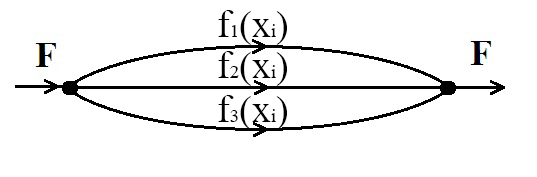
\includegraphics[width=1\linewidth]{img21.jpg}
	\caption{} \label{img:img2.1}
	\end{minipage}
	\begin{minipage}{0.43\linewidth}
	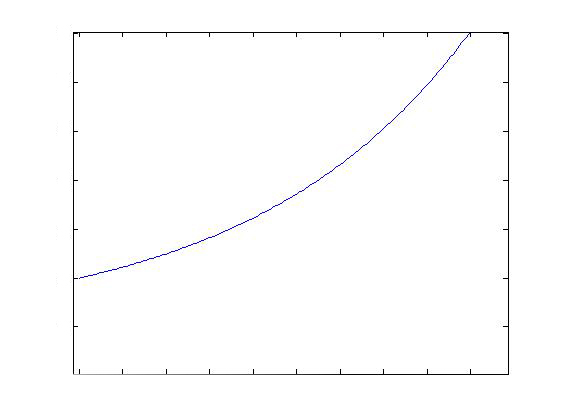
\includegraphics[width=1\linewidth]{img22.jpg}
	\caption{} \label{img:img2.2}
	\end{minipage}
\end{figure} \\

[new example]
\begin{align*}
\min\limits_x &\sum\limits_{i=1}^n f_i(x_i)x_i\\
&\sum\limits_{i=1}^n x_i = F \\
&f_i \geq 0
\end{align*}
\begin{align*}
L = \sum\limits_{i=1}^n f_i(x_i)x_i + \omega(F - \sum\limits_{i=1}^n x_i) + \sum\limits_{i=1}^n (-x_i)\eta_i
\end{align*}
\begin{align*}
\frac{\partial L}{\partial x_i} = &f_i(x_i) + \frac{\partial f_i(x_i)}{\partial x_i}x_i - \omega -\eta_i\\
&f_i(x_i) + \frac{\partial f_i(x_i)}{\partial x_i}x_i = \omega + \eta_i
\end{align*}

\begin{align*}
f_i(x_i) + \frac{\partial f_i(x_i)}{\partial x_i}x_i  \begin{cases} = \omega, \: x_i^\star > 0\\
\geq \omega, \: x_i^\star = 0
\end{cases}
\end{align*}

[рисунок перевернутой параболы]


\begin{align*}
\min\limits_x &\sum\limits_{i=1}^n \int\limits_0^{x_i} f_i(u)du\\
&\sum\limits_{i=1}^n x_i = F \\
&x_i \geq 0
\end{align*}

\begin{align*}
f_i(x_i^\star)  \begin{cases} = \omega, \: x_i^\star > 0\\
\geq \omega, \: x_i^\star = 0
\end{cases}
\end{align*}

Пусть $f_i(x_i) = a_i + b_i x_i$. Тогда

\begin{align*}
a_i + b_i x_i^\star \begin{cases} = \omega, \: x_i^\star > 0\\
\geq \omega, \: x_i^\star = 0
\end{cases}
\end{align*}
\begin{align*}
x_i^\star  \begin{cases} = \omega - a_i, \: a_i \leq \omega\\
= 0, \:a_i>\omega
\end{cases}
\end{align*}

[тут еще раз проверить с индексом к]

Перенумеруем $a_i$, чтобы $a_1 \leq a_2 \leq \dots \leq a_n$.
Существует такой номер $k$, что выполняется $a_k \leq \omega < a_{k+1}$. Тогда
\begin{align*}
&\sum \limits_{i=1}^n x_i^\star = \sum \limits_{i=1}^k x_i^\star  = \sum\limits_{i=1}^k \frac{\omega}{b_i} - \sum\limits_{i=1}^k \frac{a_i}{b_i} = F\\
&\omega = \frac{F + \sum \limits_{i=1}^k \frac{a_i}{b_i}}{\sum\limits_{i=1}^k \frac{1}{b_i}}
\end{align*}

\begin{align*}
x_i^\star = \begin{cases}
\frac{1}{b_i}\frac{F+\sum\limits_{i=1}^k \frac{a_i}{b_i}}{\sum\limits_{i=1}^k \frac{1}{b_i}} - \frac{a_i}{b_i}, \: i \leq k\\
0, \: i > k
\end{cases}
\end{align*}
Ищем $k$:
\begin{align*}
a_k \leq \frac{F+\sum\limits_{i=1}^k \frac{a_i}{b_i}}{\sum\limits_{i=1}^k \frac{1}{b_i}} < a_{k+1}
\end{align*}
\begin{align*}
a_k\sum\limits_{i=1}^k \frac{1}{b_i} - \sum\limits_{i=1}^k \frac{a_i}{b_i} \leq F < a_{k+1}\sum\limits_{i=1}^k \frac{1}{b_i} - \sum\limits_{i=1}^k \frac{a_i}{b_i}
\end{align*}


[line]

[picture]

Пусть нам известны $f_i(x_i)$, нам  нужно найти F.
Эластичный спрос

\begin{align*}
&\min\limits_x \sum\limits_{i=1}^n \int\limits_0^{x_i} f_i(u)du - \int\limits_0^F g^{-1}(\gamma)d\gamma & \\
&F - \sum\limits_{i=1}^n x_i = 0 &\omega&\\
&x_i \geq 0 &\eta_i \geq 0&
\end{align*}

\begin{align*}
L = \sum \limits_{i=1}^n \int\limits_0^{x_i} f_i(u)du - \int\limits_0^F g^{-1}(\gamma) d\gamma + \omega(F - \sum \limits_{i=1}^n x_i) + \sum\limits_{i=1} (-x_i) \eta_i
\end{align*}

\begin{align*}
& \frac{\partial L}{\partial x_i} = f_i(x_i) - \omega \eta_i = 0\\
&\frac{\partial L}{\partial F} = \omega - g^{-1}(F) = 0
\end{align*}
\begin{align*}
&f_i(x_i) = \omega+\eta_i\\
&\omega = g^{-1}(F)
\end{align*}
Пусть $g^{-1}(F) = T-F$, следовательно
\begin{align*}
&\sum \limits_{i=1}^k \frac{\omega}{b_i} - \sum \limits_{i=1}^k \frac{a_i}{b_i} = F\\
&\sum\limits_{i=1}^k \frac{\omega}{b_i} - \sum\limits_{i=1} \frac{a_i}{b_i} = T - \omega
\end{align*}
\begin{align*}
\omega = \frac{T + \sum \limits_{i=1}^k \frac{a_i}{b_i}}{1+\sum\limits{i=1}^k \frac{1}{b_i}}
\end{align*}

\begin{align*}
F =\frac{ T \sum\limits{i=1}^k \frac{1}{b_i} + \sum \limits_{i=1}^k \frac{a_i}{b_i}}{1+\sum\limits{i=1}^k \frac{1}{b_i}}
a_k \leq \frac{ T \sum\limits{i=1}^k \frac{1}{b_i} + \sum \limits_{i=1}^k \frac{a_i}{b_i}}{1+\sum\limits{i=1}^k \frac{1}{b_i}} < a_k+1
\end{align*}
T -- лояльность потребителей к потерям (задержкам).
\subsection{Задача. Первая лабораторная}
\begin{align*}
&\min \limits_x \sum \limits_{i=1}^n \int\limits_0^{x_i} f_i(u)du, \text{ где $f_i$ -- любые выпуклые функции}\\
&\sum\limits_{i=1}^n x_i =F\\
&x_i \geq 0\\
&\text{Вывод: $x$, $f_i(x_i)$.}
\end{align*}

\subsection{Метод Франка-Вульфа}
\begin{enumerate}
\item Задаем $x^0$ (например $x_i = \frac{F}{n}$), $LBD = 0$
\item $\overline{z}(x) = z(x^k)+ \triangledown z(x^k)(x-x^k)$ -- минимизируем функцию.\\
$\min \overline{z}(x)$\\
$\sum\limits_{i=1}^n x_i =F$\\
$x_i \geq 0$ \\
Получаем $y^k$. Вводим направление спуска $p^k = y^k -x^k$.
\item $LBD = \max \{LBD, \overline{z}(y^k) \}$
Критерий сходимости: $\frac{\overline{z}(x^k) - LBD}{LBD} < \varepsilon$
\item $arg\min \{z(x^k+lp^k) | 0\leq l\leq 1 \}$ -- находим длину шага
\item $x^{k+1} = x^k + l_k p^k$  -- проверяем критерий сходимости, если не выполнено то возвращаемся к шагу 2.
\end{enumerate}
\chapter{Лекция 4}


\begin{figure}[h]
	\centering
	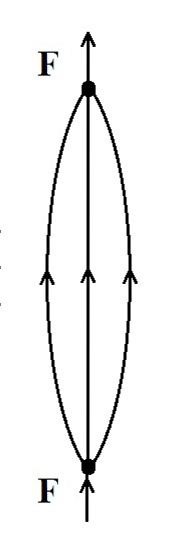
\includegraphics[width=0.1\linewidth]{img441.jpg}
	\caption{} \label{img:img44.1}
\end{figure}
$F = \sum\limits_{j=1}^m F^j$ -- имеется $m$ групп пользователей,
$F^j$ -- поток группы.\\ 
Каждая группа стремиться минимизировать совой поток:
\begin{gather*}
\min\limits_{f^j} \sum\limits_{i=1}^n t_i(f_i)f_i^j, \qquad f^j = (f_1^j, f_2^j, \dots, f_n^j) - \text{стратегия} \\
\sum\limits_{i=1}^n f_i^j = F^j, \qquad f_i = \sum\limits_{j=1}^m f_i^j
\end{gather*}

\begin{equation*}
\frac{\partial L^j}{\partial f_i^j} = t_i(f_i)+ \frac{\partial t_i(f_i)}{\partial f_i^j}f_i^j - \omega^j-\eta_i^j = 0
\end{equation*}

\begin{equation*}
t_i(f_i) + \frac{\partial t_i(f_i)}{\partial f_i^j}f_i^j \begin{cases} = \omega^j & если f_i^j > 0\\
> \omega^j & если f_i^j = 0 
\end{cases}
\end{equation*}

\begin{equation*}
t_i(f_i) = a_i + b_if_i
\end{equation*}

\begin{equation*}
a_i+b_i \sum\limits_{j=1}^m f_i^j + b_i f_i^j \begin{cases} = \omega^j & если f_i^j > 0\\
\geq \omega^j & если f_i^j = 0 
\end{cases}
\end{equation*}

\begin{equation*}
f_i^1+ \dots + 2f_i^j+ \dots +  f_i^m  \begin{cases} = \frac{\omega^j -a_i}{b_i} & если f_i^j > 0\\
\geq \frac{\omega^j -a_i}{b} & если f_i^j = 0 \text{!!!!!!!!!!!}
\end{cases}
\end{equation*}

\begin{equation*}
\begin{pmatrix}
2 & 1 & \cdots & 1\\
1 & 2 & \cdots & 1\\
\vdots & \vdots & \ddots & \vdots\\
1 & 1 & \cdots & 2 
\end{pmatrix}
\begin{pmatrix}
f_i^1 \\ f_i^2 \\ \vdots\\ f_i^m 
\end{pmatrix}
=
\begin{pmatrix}
\frac{\omega^1 - a_i}{b_i} \\ \frac{\omega^2 - a_i}{b_i} \\ \vdots \\ \frac{\omega^m - a_i}{b_i}
\end{pmatrix}
\end{equation*}
Следовательно
\begin{equation*}
\begin{pmatrix}
f_i^1 \\ f_i^2 \\ \vdots\\ f_i^m 
\end{pmatrix} 
=\begin{pmatrix}
\frac{m}{m+1} & \frac{-1}{m+1} & \cdots & \frac{-1}{m+1} \\
\frac{-1}{m+1} & \frac{m}{m+1} & \cdots & \frac{-1}{m+1} \\
\vdots & \vdots & \ddots & \vdots\\
\frac{-1}{m+1} & \frac{-1}{m+1} & \cdots & \frac{m}{m+1} \\
\end{pmatrix}
\begin{pmatrix}
\frac{\omega^1 - a_i}{b_i} \\ \frac{\omega^2 - a_i}{b_i} \\ \vdots \\ \frac{\omega^m - a_i}{b_i}
\end{pmatrix}
\end{equation*}

Для экономии времени и места обозначим $\xi_i^j = \frac{\omega^j - a_i}{b_i}$.

\begin{equation*}
f_i^j = \xi_i^j - \frac{1}{m+1} \sum\limits_{q=1}^m \xi_i^q
\end{equation*}

\begin{equation}
F^j = \sum\limits f_i^j = \sum\limits_{i=1}^n \xi_i^j - \frac{1}{m+1} \sum\limits_{i=1}^n \sum\limits_{q=1}^m \xi_i^q
\end{equation}

\begin{equation*}
\begin{pmatrix}
F^1 \\ F^2 \\ \vdots\\ F^m 
\end{pmatrix} 
=
\begin{pmatrix}
\frac{m}{m+1} & \frac{-1}{m+1} & \cdots & \frac{-1}{m+1} \\
\frac{-1}{m+1} & \frac{m}{m+1} & \cdots & \frac{-1}{m+1} \\
\vdots & \vdots & \ddots & \vdots\\
\frac{-1}{m+1} & \frac{-1}{m+1} & \cdots & \frac{m}{m+1} \\
\end{pmatrix}
\begin{pmatrix}
\sum\limits_{i=1}^n \xi_i^1 \\ \sum\limits_{i=1}^n \xi_i^2 \\ \vdots \\ \sum\limits_{i=1}^n \xi_i^m
\end{pmatrix}
\end{equation*}

\begin{equation*}
\begin{pmatrix}
\sum\limits_{i=1}^n \xi_i^1 \\ \sum\limits_{i=1}^n \xi_i^2 \\ \vdots \\ \sum\limits_{i=1}^n \xi_i^m
\end{pmatrix}
=
\begin{pmatrix}
2 & 1 & \cdots & 1\\
1 & 2 & \cdots & 1\\
\vdots & \vdots & \ddots & \vdots\\
1 & 1 & \cdots & 2 
\end{pmatrix}
\begin{pmatrix}
F^1 \\ F^2 \\ \vdots\\ F^m 
\end{pmatrix}
\end{equation*}
Отсюда

\begin{equation*}
\sum\limits_{i=1}^n\xi_i^j = F^1 + \dots + 2F^j+ \dots + F^m
\end{equation*}

\begin{equation*}
\sum\limits_{i=1}^n\frac{\omega^j - a_i}{b_i} = F^j + \sum\limits_{i=1}^m F^i
\end{equation*}

\begin{equation*}
\omega^j = \frac{F^j + \sum\limits_{i=1}^m F^i + \sum\limits_{i=1}^n  \frac{a_i}{b_i}}{\sum\limits_{i=1}^n \frac{1}{b_i}}
\end{equation*}

\begin{equation*}
\xi_i^j = \frac{1}{b_i}\frac{F^j + \sum\limits_{q=1}^m F^q + \sum\limits_{s=1}^n \frac{a_s}{b_s}}{\sum\limits_{s=1}^n \frac{1}{b_s}} - \frac{a_i}{b_i}
\end{equation*}

Если $m=1$, то
\begin{equation*}
f_i^j = \frac{1}{b_i}\frac{F+ \frac{1}{2}\sum\limits_{s=1}^n \frac{a_s}{b_s}}{\sum\limits_{s=1}^n\frac{1}{b_s}} + \frac{1}{2}\frac{a_i}{b_i}
\end{equation*}

\begin{equation*}
T^{u \varepsilon}(f_i) = \sum\limits_{i=1}^n \int\limits_0^{f_i} t_i(u)du
\end{equation*}

\begin{equation*}
T^{so}(f_i) = \sum\limits_{i=1}^n t_i(f_i)f_i
\end{equation*}


\begin{equation*}
T_m^{n \varepsilon}(f_i) = \sum\limits_{j=1}^m \sum\limits_{i=1}^n t_i(f_i)f_i^j
\end{equation*}

\begin{equation*}
T^{so} \leq T_m^{n \varepsilon} \leq T^{u \varepsilon}
\end{equation*}

\begin{equation*}
T^{so} = T_1^{n \varepsilon} \leq T_2^{n \varepsilon} \leq \dots \leq T_{|F|}^{n \varepsilon} 
= T_{\infty}^{n \varepsilon} = T^{u \varepsilon} [!!!!!!!!!!!!]
\end{equation*}


\chapter{Лекции 5-6}

\section{Двойственная задача программирования}
Рассмотрим задачу о нахождении максимума функции $f(x)$ при заданных ограничениях $g_i(x) \geqslant 0,~ i = \overline{1,m}$:
\begin{equation}\label{eq:eq1}
\max_{x \in X} f(x)
\end{equation}

\begin{equation}\label{eq:eq2}
X=\{~x~|~x \in \textit{R} ^n,~g_i(x) \geqslant 0,~i = \overline{1,m}~\},~m < n
\end{equation}

Построим функцию Лагранжа этой задачи:
\begin{equation} \label{eq:eq3}
F(x,y)=f(x)+ \sum_{i=1}^m y_i g_i(x)
\end{equation}

И поставим вопрос о поиске величины:
\begin{equation} \label{eq:eq4}
 \max_{x \in \textit{R} ^n} \min_{y \in Y} F(x,y),~ Y= \left\{~y~|~y_i \geqslant 0, ~i = \overline{1,m}\right\}
\end{equation}


\begin{definition}
Пара $(x^0,y^0)$ называется седловой точкой функции $F(x,y)$ на множестве $X \times Y$, если выполняется:
$$F(x,y^0) \leqslant F(x^0,y^0) \leqslant F(x^0,y),~ \forall x\in X,~ \forall y \in  Y $$	
\end{definition}

Иначе говоря, если точка $(x^0,y^0)$ является седловой, то
$$ \max_{x \in X}F(x,y^0) = \min_{y \in Y}F(x^0,y) = F(x^0,y^0)$$

Введем в рассмотрение величины:
$$\upsilon = \sup_{x \in X} \inf_{y \in Y} F(x,y),~\bar{\upsilon}=\inf_{y \in Y}\sup_{x \in X} F(x,y)$$

\begin{lemma} \label{lem:lem1}
$$\upsilon \leqslant \bar{\upsilon} \text{ или, что то же самое, } \sup_{x \in X} \inf_{y \in Y} F(x,y) \leqslant \inf_{y \in Y}\sup_{x \in X} F(x,y)$$
\end{lemma}

\begin{proof}
$$\upsilon = \sup_{x \in X} \inf_{y \in Y} F(x,y) \leqslant \sup_{x \in X}F(x,y'),~ \forall y' \in Y$$
и следовательно:
$$\upsilon \leqslant \inf_{y \in Y}\sup_{x \in X} F(x,y) = \bar{\upsilon}$$	

\end{proof}

\begin{theorem}
Для того, чтобы функция $F(x,y)$ имела седловую точку на множестве $(x,y) \in X \times Y$, необходимо и достаточно, чтобы выполнялось условие:
$$\max_{x \in X} \min_{y \in Y} F(x,y) = \min_{y \in Y}\max_{x \in X} F(x,y)$$
\end{theorem}

\begin{theorem}
Задачи \eqref{eq:eq1}, \eqref{eq:eq2} и \eqref{eq:eq3}, \eqref{eq:eq4} эквивалентны:  

\begin{enumerate}
\item $\bar{\upsilon} = \upsilon$;
\item $\displaystyle \max_{x \in X} f(x) =  \max_{x \in \textit{R} ^n} \min_{y \in Y} F(x,y)$.
\end{enumerate}
\end{theorem}

\begin{proof}
Введем в рассмотрение функцию $\displaystyle \varphi(x)=\inf_{y \in Y} F(x,y).$

Для любого $x \in X$ и для любого номера $i \in \{1,2,...,m\}$ справедливо неравенство $g_i(x) \geqslant 0$, поэтому $F(x,y) \geqslant f(x)$ и, соответственно, $\varphi(x) = F(x,0) = f(x),~ \forall x \in X$. 

Если же $x \notin X$, то $g(i) < 0$ хотя бы для одного номера $i \in \{1,2,...,m\}$. Построим такую последовательность векторов $\{y^k\} \in Y$, чтобы  $y_i^k \rightarrow \infty$. Тогда $F(x,y^k) \rightarrow -\infty$, из чего следует, что $\varphi(x) = -\infty,~ \forall x \notin X$.

Таким образом, если $X \neq \emptyset$, то $\displaystyle \upsilon = \sup_{x \in R} \varphi(x) = \sup_{x \in X} \varphi(x) = \sup_{x \in X} f(x) = \inf_{y \in Y}\sup_{x \in X} F(x,y) = \bar{\upsilon}$, и решения задач \eqref{eq:eq1},\eqref{eq:eq2} и \eqref{eq:eq3},\eqref{eq:eq4} могут существовать только одновременно и совпадают.

При $X = \emptyset$ обе задачи не имеют решения.
\end{proof}

\begin{definition}
Задача \eqref{eq:eq3},\eqref{eq:eq4} называется двойственной задачей по отношению к задаче \eqref{eq:eq1},\eqref{eq:eq2}. Соотношение $\upsilon = \bar{\upsilon}$ называется соотношением двойственности, а теоремы, устанавливающие это соотношение, называются теоремами двойственности. 
\end{definition}

\begin{theorem} \label{teor:teor1}
Если функция Лагранжа \eqref{eq:eq3} имеет седловую точку на $\textit{R}^n \times Y$, то выполняется соотношение двойственности: пусть точка $(x^0,y^0)$ является седловой, тогда $x^0$ соответствует решению задачи \eqref{eq:eq1}, \eqref{eq:eq2}, а $y^0$ задачи \eqref{eq:eq3}, \eqref{eq:eq4}.

\end{theorem}

\section{Задача выпуклого программирования}

\begin{definition}
Функция $f(x)$ называется выпуклой на $X$, если $\forall x',x'' \in X$ выполняется соотношение:
$$f(\lambda x' + (1-\lambda)x'') \leqslant \lambda f(x') + (1-\lambda) f(x''), \forall \lambda \in [0,1]$$
\end{definition}

Аналогично вводится определение вогнутой функции.

\begin{definition}
	Функция $f(x)$ называется вогнутой на $X$, если $\forall x',x'' \in X$ выполняется соотношение:
	$$f(\lambda x' + (1-\lambda)x'') \geqslant \lambda f(x') + (1-\lambda) f(x''), \forall \lambda \in [0,1]$$
\end{definition}

\begin{definition}
Задачей выпуклого программирования называется задача \eqref{eq:eq1}, \eqref{eq:eq2} при условии, что $f(x)$ и $g_i(x)$ -- вогнутые функции.
\end{definition}

\begin{lemma}
Множество допустимых решений задачи выпуклого программирования \ref{eq:eq1}, \ref{eq:eq2} является выпуклым. Любой локальный максимум является глобальным.
\end{lemma}

\begin{proof}
Пусть $x',x'' \in X$, т. е. $g_i(x') \geqslant 0$, $g_i(x'') \geqslant 0$, $i = \overline{1,m}$. Рассмотрим значение функций $g_i(x)$ в точке $x = \lambda x' + (1-\lambda) x''$:
$$g_i(x) = g_i(\lambda x'  + (1-\lambda) x'') \geqslant \lambda g_i(x') + (1-\lambda) g_i(x'') \geqslant 0$$
Следовательно $x$ также принадлежит $X$, и $X$ -- выпуклое множество.

Пусть $x^*$ -- точка локального максимума. Это значит, что $f(x) \geqslant f(x),~ \forall x \in X \cap S(x^*,\varepsilon)$, где $S(x^*,\varepsilon)$ -- малая окрестность точки $x^*$.

Предположим, что существует точка $\hat{x} \in X$ и $f(\hat{x})>f(x^*)$. Тогда для точки $\tilde{x} = \lambda x^* + (1-\lambda) \hat{x},~\lambda \in (0,1)$ справедливо:
$$f(\tilde{x}) \geqslant \lambda f(x^*)+ (1-\lambda) f(\hat{x}) > \lambda f(x^*) + (1-\lambda)f(x^*) = f(x^*)$$
и существует такое $\lambda \in (0,1)$, что $\tilde{x}(\lambda) \in X \cap S(x^*,\varepsilon)$. Получаем противоречие, указывающее на ошибочность сделанного предположения. 

Значит, для любой точки $x \in X$ выполняется соотношение $f(x) \leqslant f(x^*)$, что соответствует определению глобального максимума в точке $x^*$. 
\end{proof}

\begin{theorem}
Пусть $X$ и $Y$ -- выпуклые, замкнутые и ограниченные подмножества евклидова пространства, а функция $F(x,y) \in C(X \times Y)$ вогнута по $x,~\forall y \in Y$, и выпукла по $y,~\forall x \in X$. Тогда $F(x,y)$ имеет седловую точку на $X \times Y$. 
\end{theorem}

\begin{definition}
Задача выпуклого программирования удовлетворяет условию Слейтера, если $\exists x \in \textit{R}^n:~g_i(x)>0,~i=\overline{1,m}$.
\end{definition}

\begin{theorem}
Если задача выпуклого программирования удовлетворяет условию Слейтера, то необходимым и достаточным условием оптимальности точки $x^0$ в задаче \eqref{eq:eq1}, \eqref{eq:eq2} является существование такого вектора $y^0 \in Y$, чтобы точка $(x^0,y^0)$ была седловой для \eqref{eq:eq3}.
\end{theorem}

\begin{proof}~
		
\emph{Достаточность} следует из теоремы \ref{teor:teor1}.

\emph{Необходимость.} Введем в рассмотрение следующие множества:

\begin{align*}
A &= \left\{z = (z_1,z_2,...,z_m,z_{m+1})^T|~z_i \leqslant g_i(x),~i = \overline{1,m},~z_{m+1} \leqslant f(x) \right\}, \\
B &= \left\{z = (z_1,z_2,...,z_m,z_{m+1})^T|~z_i > 0,~i = \overline{1,m},~z_{m+1} >f(x^0) \right\},
\end{align*}
где $x^0$ -- решение задачи выпуклого программирования, а $x$ -- произвольная точка множества $\textit{R}^n$.

Покажем, что множествл $A$ является выпуклым. Пусть
$$z',z'' \in A \Rightarrow z' \leqslant g_i(x'),~ z'' \leqslant g_i(x''),~ z_{m+1}' \leqslant f(x'),~z_{m+1}'' \leqslant f(x'')$$

Рассмотрим точку $z^\alpha = \alpha z' + (1-\alpha)z''$.
$$z_i^\alpha \leqslant \alpha g_i(x') + (1-\alpha)g_i(x'') \leqslant g_i(\alpha x' + (1+\alpha) x'') = g_i(x^\alpha),$$
где $x^\alpha = \alpha x' + (1+\alpha) x''$, $i=\overline{1,m}$
$$z_{m+1}^\alpha \leqslant \alpha f(x') + (1-\alpha)x'' \leqslant f(x^\alpha),$$
т.е. $z^\alpha \in A$, поэтому $A$ -- выпуклое множество.

Множество $B$ представляет собой открытый ортант с вершиной в точке $(0,0,...,f(x^0))^T$, поэтому $B$ также выпукло.

В силу оптимальности вектора $x^0$ множества $A$ и $B$ не пересекаются, т. е. $A \cap B = \emptyset$. Значит, по теореме о разделяющей гиперплоскости существует такой ненулевой вектор $a = (a_1,a_2,...,a_{m+1})^T$, что

\begin{equation}\label{eq:eq5}
(a,z^1) \leqslant (a,z^2),~ \forall z^1 \in A, z^2 \in B
\end{equation}

Предположим, что $a_i < 0$, тогда, выбирая последовательность $\{z^k\} \in B$ таким образом, чтобы $z_i^k \rightarrow \infty$, а остальные компоненты были равны нулю, получим $(a,z^k) \rightarrow -\infty$, что противоречит неравенству \eqref{eq:eq5}, следовательно предположение неверно. 

Так как точка $(0,0,...,f(x^0))^T$ является предельной для множества $B$, то выполняется неравенство:
\begin{equation}\label{eq:eq6}
\sum_{i=1}^m a_i g_i(x) + a_{m+1} f(x) \leqslant a_{m+1} f(x^0)
\end{equation}

Поэтому $a_{m+1}>0$, поскольку, если $a_{m+1}=0$, то из \eqref{eq:eq6} получаем $\sum_{i=1}^m a_i g_i(x) \leqslant 0,\forall x \in X$, что противоречит условию Слейтера. \vspace{1ex}

Положим $\displaystyle y_i^0 = \frac{a_i}{a_{m+1}},~ i=\overline{1,m}$, тогда из \eqref{eq:eq6} следует: 
\begin{equation} \label{eq:eq7}
\sum_{i=1}^m y_i^0 g_i(x) + f(x) \leqslant f(x^0),~\forall x \in \textit{R}
\end{equation}

При $x = x^0$ получаем $\displaystyle  \sum_{i=1}^m y_i^0 g_i(x^0) \leqslant 0$. Но $\displaystyle y_i^0 \geqslant 0,~g_i(x^0) \geqslant 0 \Rightarrow \sum_{i=1}^m y_i^0 g_i(x^0) \geqslant 0$. Значит

\begin{equation} \label{eq:eq8}
\sum_{i=1}^m y_i^0 g_i(x^0) = 0
\end{equation}

Прибавив эту сумму к правой части \eqref{eq:eq7}, получим: $F(x,y^0) \leqslant F(x^0,y^0),\forall x \in X$.



Поскольку $\displaystyle  \sum_{i=1}^m y_i g_i(x^0) \geqslant 0, \forall y \geqslant 0$, имеем  $F(x^0,y^0) \leqslant F(x^0,y),\forall y \geqslant 0$. Значит, $(x^0,y^0)$ -- седловая точка.
\end{proof}

\begin{definition}
Ограничения, которые выполняются в некоторой точке как равенства называются активными. Множество $I(x) = \{~i~|~1\leqslant i \leqslant m,~g_i(x)=0\}$ - совокупность индексов активных ограничений.
\end{definition}

Из свойства \eqref{eq:eq8} седловой точки получаем, что $y_i^0 = 0, \forall i \notin I(x^0)$. Поэтому для определения $x^0$ и ненулевых $y_i^0$ имеем систему:

\begin{equation} \label{eq:eq9}
\begin{cases} 
\displaystyle \frac{\partial f(x)}{\partial x_j} + \sum_{i \in I(x^0)} y_i^0 \frac{\partial g_i(x^0)}{\partial x_j} = 0,\\[3ex]
g_i(x^0) = 0,~i \in I(x^0)
\end{cases}
\end{equation}

\begin{theorem}
Система \eqref{eq:eq9} представляет собой необходимые и достаточные условия оптимальности для задачи выпуклого программирования в случае, когда $R=\textit{R}^n$.
\end{theorem}

\begin{theorem}
Необходимые и достаточные условия оптимальности для задачи выпуклого программирования в случае $R = \{~x~|~x \geqslant 0\}$ можно представить в виде системы:

$$
\begin{cases} 
\frac{\partial F(x^0,y^0)}{\partial x_j} \leqslant 0,~j=\overline{1,n},\\[2ex]
\displaystyle \sum_{j=1}^n \frac{\partial F(x^0,y^0)}{\partial x_j} x_j^0 = 0,\\[3ex]
g_i(x^0) y_i^0 = 0,~i=\overline{1,m}.
\end{cases} 
$$ 
\end{theorem}

Рассмотрим более общую задачу о поиске
$$max_{x \in \textit{R}^n} f(x)$$
при ограничениях
$$g_i(x) \geqslant 0,~i=\overline{1,m}$$
$$H_k(x)=0,~k=\overline{1,r}$$

Для данной задачи справедлива следующая теорема.

\begin{theorem}
Если $f(x)$ и $g_i(x)$ -- вогнутые на гиперплоскости, определяемой уравнениями $H_k(x) = 0, ~i=\overline{1,m}$, и на этой гиперплоскости выполняются условия Слейтера, то решение $x^0$ существует и является глобальным максимумом. При этом для функции Лагранжа $\displaystyle L(x,y,\nu) = f(x) + \sum_{i=1}^m y_i g_i(x) - \sum_{k=1}^r \nu_k H_k(x)$ существуют такие $y_i^0 \geqslant 0,~i=\overline{1,m}$ и $\nu_k^0,~k=\overline{1,r}$, что в точке $(x^0,y^0,\nu^0)$ выполняются следующие условия:

$$
\begin{cases}
\displaystyle \frac{\partial L}{\partial x_j} = 0,~j=\overline{1,n},\\[2ex]
\displaystyle \frac{\partial L}{\partial y_i} \geqslant 0,~i=\overline{1,m},\\[2ex]
\displaystyle y_i^0 \frac{\partial L}{\partial y_i} = 0,~i=\overline{1,m},\\[2ex]
\displaystyle \frac{\partial L}{\partial \nu_k} = 0,~k=\overline{1,r},\\
\end{cases}
$$

\end{theorem}

\begin{example}
На предприятии имеется два вида ресурсов. Цена ресурса первого вида 3 единицы, второго -- 4 единицы. Известно, что из $x_1$ первого ресурса и  $x_2$ второго ресурса можно получить $z(x_1,x_2) = \sqrt{x_1^2 + x_2^2}$ единиц продукта. Какое распределение ресурсов будет оптимальным, если всего на производство выделено 24 единицы?

\begin{figure}[h]
	\centering
	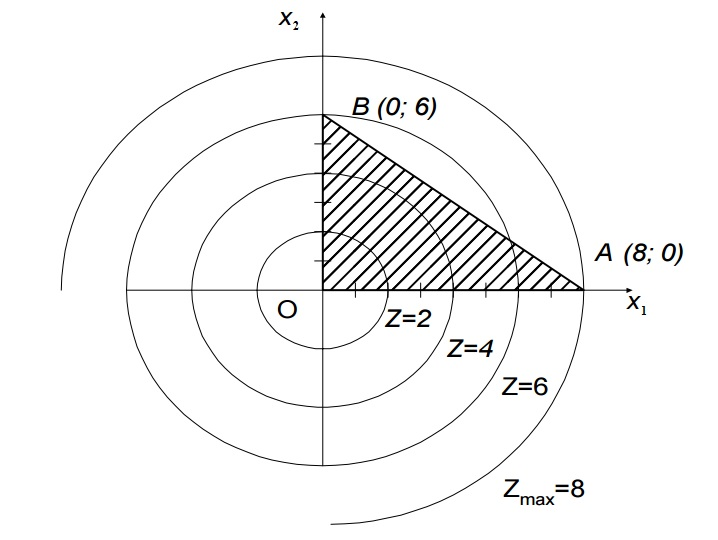
\includegraphics[width=0.43\linewidth]{img41.jpg}
	\caption{} \label{img:img4.1}
\end{figure}

Математическая модель задачи выглядит следующим образом:
\begin{equation*}
\begin{aligned}
z(x^0) = \max_x \sqrt{x_1^2+x_2^2},\\
3x_1+4x_2 \leqslant 24, \\
x_1 \geqslant 0,~x_2 \geqslant 0
\end{aligned}
\end{equation*}
\end{example}

Множество допустимых решений заштриховано на рис. \ref{img:img4.1}. Если целевой функции придавать фиксированные значения 1, 2, 3, \dots, то будем получать окружности с центром в начале координат и радиусом 1, 2, 3, \dots~. Начертим ряд окружностей (линии уровня целевой функции). Из рисунка видно, что функция $z(x_1,x_2)=\sqrt{x_1^2+x_2^2}$ достигает наибольшего значения, равного 8, в точке $А(8; 0)$, т.е. $z_{\max}=z(8; 0)=8$.

\section{Численные методы решения задач нелинейного программирования с ограничениями}

В зависимости от наличия ограничений градиентные методы модифицируются путем проекции полученного нового приближения на допустимое множество значений $x \in X$:
\begin{enumerate}
\item Градиентные методы: 
$$ x^{k+1} = x^k +\alpha_k f'(x^k) \text{, где } f(x^k + \alpha_k f'(x^k)) = \max_{\alpha \geqslant 0} f(x^k + \alpha f'(x^k));$$
\item Проективные методы:
$$x^{k+1}=P_x(x^k + \alpha_k f'(x^k)).$$
\end{enumerate}

\chapter{Лекция 7}
\begin{align*}
&\min \sum\limits_{i=1}^n \int_{0}^{f_i} t_i(u)du\\
&a_i(f_i)=t_i(f_i)-t_i^{\prime} (f_i)f_i\\
&b_i(f_i)=t_i^{\prime} (f_i)\\
&\sum\limits_{i=1}^n\ f_i=F\\
&f_i \geqslant 0, \forall i= \overline{1,n}\\
\end{align*}

$f_i^k$: перенумеруем $f_i, u_i, b_i, t_i$ так, чтобы $a_1(f_1^k)\leqslant...\leqslant a_n(f_n^k)$. Мы их перенумеровываем каждый раз все. Далее находим $m^k$ - количество не нулевых $f_i.$ \\
\begin{align*}
\omega^k=\dfrac{F+\sum \limits_{i=1}^n\dfrac{a_i(f_i^k)}{b_i(f_i^k)}}{\sum \limits_{i=1}^{m^n} \dfrac{1}{b_i(f_i^k)}}
\end{align*}
$a_{m^k}(f_{m^k}^k) \leqslant \omega^k \textless a_{m^{k+1}}( f_{m^{k+1}}^k) $

Как только находим $m^k$ ищем 
\begin{equation*}
f_i^{k+1} = 
 \begin{cases}
  \dfrac{ \dfrac{1}{b_i(f_i^k)} (F+\sum \limits_{s=1}^{m^k} \dfrac{a_s(f_s^k)}{b_s(f_s^k)})}{\sum \limits_{s=1}^{m^n} \dfrac{1}{b_s(f_s^n)}} - \dfrac{a_i(f_i^k)}{b_i(f_i^k)}, \:  i\leqslant m^k\\
   0, \:  {i>m^k}\\
 \end{cases}
\end{equation*}

Предложение: на первом шаге взять $f_i^0 = \dfrac{F}{n}, \forall i=\overline{1,n}$

Для простоты будем рассматривать вариант $ m^n=m^* $.\\
Рассмотрим $f_i^{k+1}-f_i^*=f_i^k-\dfrac{t_i(f_i^k)}{t_i^{\prime} (f_i^k)}+\dfrac{F-\sum\limits_{s=1}^m \left[ f_s^k-\dfrac{t_s^k(f_s^k)}{t_s^{\prime} (f_s^k)}\right]}{\sum \limits_{s=1}^m \dfrac{t_i^{\prime} (f_i^k)}{t_s^{\prime} (f_s^k)}}-f_i^* $. Далее разложим $F$ и внесем под сумму. 

\begin{align*}
f_i^{k+1}-f_i^*=(f_i^k-f_i^*) - \dfrac{t_i(f_i^k)-t_i(f_i^*)}{t_i^{\prime} (f_i^k)}  - \dfrac{t_i(f_i^*)}{t_i^{\prime} (f_i^k)}- \dfrac{\sum \limits_{s=1}^m \left[ f_s^k-f_s^*-\dfrac{t_s(f_s^k)-t_s(f_s^*)}{t_s^{\prime} (f_s^k)}-\dfrac{t_s(f_s^*)}{t_i^{\prime} (f_i^k} \right ]}{\sum \limits_{s=1}^m \dfrac{t_i^{\prime} (f_i^k)}{t_s^{\prime} (f_s^k)}}
\end{align*}


Теперь, пользуясь замечательным свойством $ t_i(f_i^\star)=\omega, \: \forall i $\\
\begin{multline*}
f_i^{k+1}-f_i^*=(f_i^k-f_i^*)-\dfrac{t_i(f_i^k)-t_i(f_i^*)}{t_i^{\prime} (f_i^k)} - \dfrac{\omega}{t_i^{\prime} (f_i^k)}- \dfrac{\sum \limits_{s=1}^m \left[ f_s^k-f_s^*-\dfrac{t_s(f_s^k)-t_s(f_s^*)}{t_s^{\prime} (f_s^k)}-\dfrac{\omega}{t_i^{\prime} (f_i^k)} \right]}{\sum \limits_{s=1}^m \dfrac{t_i^{\prime} (f_i^k)}{t_s^{\prime} (f_s^k)}}=\\
=(f_i^k-f_i^*)-\dfrac{t_i(f_i^k)-t_i(f_i^*)}{t_i^{\prime} (f_i^k)} - \dfrac{\omega}{t_i^{\prime} (f_i^k)}- \dfrac{\sum \limits_{s=1}^m \left[ f_s^k-f_s^*-\dfrac{t_s(f_s^k)-t_s(f_s^*)}{t_s^{\prime} (f_s^k)}\right ]-\omega \sum \limits_{s=1}^m\dfrac{1}{t_i^{\prime} (f_i^k)} }{t_i^{\prime} (f_i^k)\sum \limits_{s=1}^m \dfrac{1}{t_s^{\prime} (f_s^k)}}
\end{multline*}

\begin{multline*}
f_i^{k+1}-f_i^*=(f_i^k-f_i^*)-\dfrac{t_i(f_i^k)-t_i(f_i^*)}{t_i^{\prime} (f_i^k)} - \dfrac{\omega}{t_i^{\prime} (f_i^k)}- \dfrac{\sum \limits_{s=1}^m \left[ f_s^k-f_s^*-\dfrac{t_s(f_s^k)-t_s(f_s^*)}{t_s^{\prime} (f_s^k)}\right ] }{\sum \limits_{s=1}^m \dfrac{t_i^{\prime} (f_i^k)}{t_s^{\prime} (f_s^k)}}+\dfrac{\omega}{t_i^{\prime} (f_i^k)}
\end{multline*}

Воспользуемся разложением Лагранжа
\begin{align*}
f_i^{k+1}-f_i^*=(f_i^k-f_i^*)-\dfrac{t_i^{\prime} (\theta_i^k)}{t_i^{\prime} (f_i^k)}(f_i^k-f_i^*) - \dfrac{\sum \limits_{s=1}^m \left[ f_s^k-f_s^*-
\dfrac{t_s^{\prime} (\theta_s^k)}{t_s^{\prime} (f_s^k)}(f_s^k-f_s^*)\right ] }
{t_i^{\prime} (f_i^k)\sum \limits_{s=1}^m \dfrac{1}{t_s^{\prime} (f_s^k)}}
\end{align*} 


\begin{align*}
f_i^{k+1}-f_i^*=\left[1-\dfrac{t_i^{\prime} (\theta_i^k)}{t_i^{\prime} (f_i^k)} \right](f_i^k-f_i^*)- \dfrac{\sum \limits_{s=1}^m \left[1-
\dfrac{t_s^{\prime} (\theta_s^k)}{t_s^{\prime} (f_s^k)}(f_s^k-f_s^*)\right ] }
{t_i^{\prime} (f_i^k)\sum \limits_{s=1}^m \dfrac{1}{t_s^{\prime} (f_s^k)}}
\end{align*} 

Далее обозначим $g_i^k=1-\dfrac{t_i^{\prime} (\theta_i^k)}{t_i^{\prime} (f_i^k)}$;
$ \mathscr{L}=t_i^{\prime}(f_i^k) \sum \limits_{s-1}^m \dfrac{1}{t_s^{\prime} (f_s^k)} $;

\begin{align*}
&|f_i^k-f_i^*|\leqslant |g_i^k||f_i^k-f_i^*|+\dfrac{\left  |\sum \limits_{i=1}^m d_s^k(f_s^k-f_s^*)\right | }{|\mathscr{L}_i^k|}\\
& \sum \limits_{i=1}^m|f_i^{n+1}-f_i^*| \leqslant \sum \limits_{i=1}^m|g_i^k||f_i^k-f_i^*|+\sum\limits_{i=1}^m \dfrac{1}{|\mathscr{L}_i^k|} \left|\sum \limits_{s=1}^m(f_s^k-f_s^*)\right| \: \text {Отсюда получаем}\\
&\sum \limits_{i=1}^m |f_i^k-f_i^*| \leqslant 2\sum \limits_{i=1}^m |g_i||f_i^k-f_i^*| 
\end{align*}
 Значит, следующий шаг ограничен сверху $ \forall  \varepsilon \: \exists  \rho: f_i^k \in S_\rho(f^*); \\ $
 $ \sum \limits_{i=1}^m |f_i^{k+1}-f_i^*|\leqslant \varepsilon \sum \limits_{i=1}^m |f_i^k-f_i^*|< \varepsilon^{k+1}\sum \limits_{i=1}^m |f_i^0-f_i^k|  $

Теперь покажем, что $ |f_i^{k+1}-f_i^*| \leftrightarrow |f_i^k-f_i^*|^2$


\begin{align*}
&t_i(f_i)=t_i(f_i^*)+ t_i^{\prime} (f_i^\star)(f_i^k-f_i^*)+ \dfrac{t_i'' (f_i^k)}{2} (f_i^k-f_i^*)^2\\
&t_i(f_i^k)=\omega+ t_i^{\prime} (f_i^\star)(f_i^k-f_i^*)+ \dfrac{t_i'' (f_i^k)}{2} (f_i^k-f_i^*)^2\\
&\dfrac{t_i(f_i^k)}{t_i'(f_i^*)} = \dfrac{\omega}{t_i'(f_i^*)}+(f_i^k-f_i^*)+\dfrac{t_i''(f_i^*)}{2t_i'(f_i^*)}(f_i^k-f_i^*)^2\\
&(f_i^k-f_i^*)-\dfrac{t_i(f_i^k)}{t_i'(f_i^*)}=-\dfrac{t_i''(f_i^*)}{2t_i'(f_i^*)}(f_i^k-f_i^*)^2-\dfrac{\omega}{t_i'(f_i^*)}\\
&f_i^{k+1}-f_i^*=(f_i^k-f_i^*)-\dfrac{t_i(f_i^k)}{t_i(f_i^*)}-\dfrac{\sum \limits_{s=1}^m[\dots]}{\sum \limits_{s=1}^m\dfrac{t_i'(f_i^*)}{t_s'(f_f^k)}}\\
&f_i^{k+1}-f_i^*=-\dfrac{\omega}{t_i'(f_i^*)}-\dfrac{t_i''(f_i*)}{2t_i'(f_i^*)}\\
&|f_i^{k+1}-f_i^*| \leqslant \left | \dfrac{t_i''(f_i^*)}{2t_i(f_i^*)} \right | \left | f_i^k-f_i^*\right |^2  +\left |\dfrac{\sum \limits_{s=1}^m[\dots[!!!!!]]}{\sum \limits_{s=1}^m \dfrac{t_i'(f_i^*)}{t_s'(f_s^k)}}  \right |\\
& \sum \limits_{i=1}^m \left | f_i^{k+1}-f_i^*\right | \leqslant \frac{3}{2} \sum \limits_{i=1}^m  \left | \dfrac{t_i''(f_i^*)}{t_i'(f_i^*)}  \right |  \left | f_i^k-f_i^* \right |^2\\
\end{align*}
\chapter{Лекции 8-9}
\section{Дуополия Курно (1838 г.)}
Некоторый продукт выпускается двумя фирмами. Фирма I выпускает $q_1$ единиц продукта, фирма II выпускает $q_2$ единиц продукта. Пусть $p$ -- некоторая начальная цена продукта, a $c$ -- его себестоимость.

Тогда прибыли фирм равны, соответственно:
\begin{align*}
B_1(q_1,q_2)=(p-q_1-q_2)q_1-cq_1\\
B_2(q_1,q_2)=(p-q_1-q_2)q_2-cq_2
\end{align*}

Найдем равновесное состояние системы:
\begin{equation*}
\begin{cases}
\displaystyle \frac{\partial B_1(q_1,q_2)}{\partial q_1} = 0 \\[3ex]
\displaystyle \frac{\partial B_2(q_1,q_2)}{\partial q_2} = 0 \\
\end{cases} 
\Longrightarrow
\begin{cases}
p - c -2q_1 -q_2 = 0 \\
p - c- 2q_2 -q_1 = 0
\end{cases} 
\Longrightarrow
\begin{cases}
\displaystyle q_1=\frac{p-c-q_2}{2}\\[3ex]
\displaystyle q_2=\frac{p-c-q_1}{2}
\end{cases}
\end{equation*}

Подставим выражение для $q_1$ во второе уравнение:
$$q_2 = \frac{p - c}{2} - \frac{p-c-q_2}{4} \Rightarrow q_2 = \frac{p-c}{3} \Rightarrow q_1 = \frac{p-c}{3}$$

\section{Более сложные модели производства}
Пусть $n$ производителей выпускает $m$ видов продуктов. Величина $x_{ij}$ показывает, сколько единиц продукта $j$ выпускает (потребляет, если величина $x_{ij}$ отрицательная) производитель $i$.

Предполагается, что каждого товара выпускается не меньше, чем потребляется:
\begin{equation} \label{eq:eq5.1}
\sum_{i=1}^n x_{ij} \geqslant 0,j=\overline{1,m}
\end{equation}

Обозначим $x_i = (x_{i1},x_{i2}, ..., x_{im})^T$ производственный план фирмы $i$. Введем в рассмотрение для каждой фирмы функцию полезности производственного плана $f_i(x_i)$.

\begin{definition}
Набор $x_1^*, ..., x_n^*$ является Парето-оптимальным, если выполняется:
\begin{enumerate}
\item $\forall i:f_i(x_i^*) = f_i(\hat{x}_i),\forall \hat{x}_i$\\[1ex]
или
\item $\exists i:f_i(x_i^*) > f_i(\hat{x}_i),\forall \hat{x}_i$
\end{enumerate}
\end{definition}

Пусть $p=(\pi_1,\pi_2, ..., \pi_m)^T$ -- вектор стоимости продуктов. Поставим задачу максимизации функции полезности фирмы $i$ при условии неубыточности производства.

\begin{equation}\label{eq:eq5.2}
\begin{cases}
\displaystyle \max_{x_i} f_i(x_i)\\[2ex]
(p, x_i) \geqslant 0
\end{cases}
\end{equation}

Пусть $x_i(p)$ -- решение \eqref{eq:eq5.2}.

\begin{definition}
Решение \eqref{eq:eq5.2}: $p^*,x_1^*(p^*),x_2^*(p^*),...,x_n^*(p^*)$, удовлетворяющее \eqref{eq:eq5.1}, называется балансовым равновесием.
\end{definition}

Сделаем следующие предположения:
\begin{enumerate} \label{en:en1}
\item $\forall i~x_i \in X_i$, где $X_i$ - выпуклое, замкнутое, ограниченное множество;
\item Пусть $\displaystyle P = \left\{(\pi_1,...,\pi_m)^T|\sum_{j=1}^m \pi_j = 1, \pi_j \geqslant 0, j=\overline{1,m}\right\}$ -- симлекс в $\textit{R}^m$, тогда: $$\exists p \in P: \forall i~\exists x_i \in X_i: (p,x_i)>0;$$
\item $\forall i:~f_i(x_i)$ -- вогнутые.
\end{enumerate}

\begin{theorem}
Пусть вышеуказанные предположения справедливы, тогда существует единственное решение \eqref{eq:eq5.2}, удовлетворяющее \eqref{eq:eq5.1}.
\end{theorem}

\begin{definition}~
	
\begin{enumerate}
\item Отображение $g(x)$ переводит $X$ в себя, если $\forall x \in X~ g(x) \in X$;
\item Отображение $g(x)$ непрерывно в точке $\bar{x}$, если $\forall \{x_i\}: x_i \underset{i \to \infty}{\longrightarrow} \bar{x}$ выполняется $g(x_i) \underset{i \to \infty}{\longrightarrow} g(\bar{x})$;
\item Отображение $g(x)$ непрерывно на $X$, если $g(x)$ непрерывно во всех $x \in X$;
\item Точка $x^0 \in X$ называется неподвижной точкой множества $X$ относительно отображения $g(x)$, если $g(x^0) = x^0$.
\end{enumerate}
\end{definition}

\begin{theorem}[Брауэра]
Пусть $X$ -- выпуклое, замкнутое, ограниченное множество, $g(x)$ переводит $X$ в себя. Тогда существует неподвижная точка.
\end{theorem}

\begin{lemma}[!!!!!!!]
Пусть $X$ выпуклое, замкнутое, ограниченное множество, $z(x)$ переводит $X$ в себя. Пусть $\exists p \in P:~ (z(x),p) \geqslant 0,~p=p(x)$. Тогда $z(x) \geqslant 0$.
\end{lemma}
\begin{proof}
$z(x)=(z_1(x),...,z_m(x))^T$. Введем в рассмотрение также отображение $r(p)=(r_1(p),...,r_m(p))^T$, где $\displaystyle r_i(p)=\frac{\pi_i + \max\{0,-z_i(x)\}}{\sum_{j=1}^m \pi_j + \sum_{j=1}^m \max \{0, -z_j(x)\}}$
	
$$\sum_{i=1}^m r_i(p)=1,~r(p) \in P \Longrightarrow \exists \hat{p}:r(\hat{p})=\hat{p} \text{ (по теореме Брауэра)}$$
$$\hat{\pi}_i = \frac{\hat{\pi}_i + \max\{0,-z_i(\hat{p})\}}{\sum_{j=1}^m \hat{\pi}_j + \sum_{j=1}^m \max \{0, -z_j(\hat{p})\}}$$
$$\max\{0,-z_i(\hat{p})\} = \hat{\pi}_i \sum_{j=1}^m \max \{0, -z_j(\hat{p})\}$$
$$\sum_{i=1}^m z_i(\hat{p}) \max\{0,-z_i(\hat{p})\} = (\hat{p},z(\hat{p})) \sum_{j=1}^m \max \{0, -z_j(\hat{p})\}$$

Если $\exists z_i(x\hat{p}<0$, то приходим к противоречию.
\end{proof}


\begin{lemma}
Пусть $X_i$ - выпуклое, замкнутое, ограниченное множество, $i=\overline{1,n}$.
Тогда: 
\begin{enumerate}
\item Cуществует единственное решение $x_i(p^*)$  задачи \eqref{eq:eq5.2}, удовлетворяющее \eqref{eq:eq5.1};
\item $x_i(p^*)$ является непрерывным отображением симплекса $P$ в $\textit{R}^m$.
\end{enumerate}

\end{lemma}

\begin{proof}
Единственность решения $x_i(p^*)$ является следствием вогнутости $f_i(x_i)$ и выпуклости $X_i$

Докажем непрерывность. Предположим, что $\displaystyle \exists\{p_k\}:\lim_{k \to \infty} p_k= \bar{p}$, но при этом $\displaystyle \lim_{k \to \infty} x_i(p_k) = \hat{x}_i \neq x_i(\bar{p})$.

$$(x_i(p_k),p_k) \geqslant 0~\forall k \Longrightarrow (\hat{x}_i,\bar{p}) \geqslant 0$$ 
при этом $f_i(x_i(\bar{p})) > f_i(\hat{x}_i) \Longrightarrow \exists \alpha: f_i(\hat{x}_i) <f_i(x_i(\bar{p})) - \alpha$. Значит, для достаточно больших номеров $k$ справедливо соотношение: 
\begin{equation} \label{eq:eq5.3}
f_i(x_i(p_k)) <f_i(x_i(\bar{p})) - \frac{\alpha}{2}
\end{equation}
следовательно:
\begin{equation} \label{eq:eq5.4}
(p_k,x_i(\bar{p}))<0 \text{ (в силу единственности решения)}
\end{equation}
$$\lim_{k \to \infty} (p_k,x_i(\bar{p})) = (\bar{p},x_i(\bar{p})) \leqslant 0 \Longrightarrow (\bar{p},x_i(\bar{p})) = 0$$
\begin{equation} \label{eq:eq5.5}
\lim_{k \to \infty}(p_k,x_i(\bar{p}))=0
\end{equation}

Согласно предположению $2$ на стр. \pageref{en:en1}: $\exists \tilde{x}_i \in X_i: (\bar{p},\tilde{x}_i) >0$, а значит:
\begin{equation} \label{eq:eq5.6}
(p_k,\tilde{x}_i)>\frac{(\bar{p},\tilde{x}_i)}{2} >0
\end{equation}

Покажем, что \eqref{eq:eq5.3}, \eqref{eq:eq5.4}, \eqref{eq:eq5.5}, \eqref{eq:eq5.6} одновремененно невозможны.

Пусть $x_i^k = x_i(\bar{p}) + \lambda_k (\tilde{x}_i - x_i(\bar{p}))$, где $\lambda_k \ \in (0,1)$ выбирается из условия $(p_k,x_i^k) = 0$:
$$\lambda_k = - \frac{(p_k,x_i(\bar{p}))}{(p_k,\tilde{x}_i) - (p_k,x_i(\bar{p}))}$$

Значит, $x_i^k$ принадлежит отрезку между $x_i(\bar{p})$ и $\tilde{x}_i$, следовательно $x_i^k \in X_i$.
При этом $\displaystyle \lim_{k \to \infty} \lambda_k = 0$ (согласно \eqref{eq:eq5.5}).
$$f_i(x_i^k) \leqslant f_i(x_i(p^k))$$
$$f_i(x_i^k) \geqslant f_i(x_i(\bar{p})) + \lambda_k (f_i(\tilde{x}_i) - f_i(x_i(\bar{p}))$$
$$f_i(x_i^k)> f_i(x_i(p_k)) + \frac{\alpha}{2}$$

Получаем противоречие.
\end{proof}

\section{Дуополия Бертрана (1883 г.)}
Две фирмы выпускают взаимозаменяемые продукты. Фирма I продает свой продукт по цене $q_1$, фирма II продает по цене $q_2$. Пусть $k$ -- коэффициент взаимозаменяемости продуктов, a $c$ -- их себестоимость, $d$ -- начальный спрос.

Тогда прибыли фирм равны, соответственно:
\begin{align*}
H_1(q_1,q_2) = (d-q_1 +kq_2)(q_1-c) \\
H_2(q_1,q_2) = (d-q_2 +kq_1)(q_2-c)
\end{align*}

Найдем равновесное состояние системы:
\begin{equation*}
\begin{cases}
\displaystyle \frac{\partial H_1(q_1,q_2)}{\partial q_1} = 0 \\[3ex]
\displaystyle \frac{\partial H_2(q_1,q_2)}{\partial q_2} = 0 \\
\end{cases} 
\Longrightarrow
\begin{cases}
d + c -2q_1 +kq_2 = 0 \\
d + c -2q_2 +kq_1 = 0
\end{cases} 
\Longrightarrow
\begin{cases}
\displaystyle q_1=\frac{d+c+kq_2}{2}\\[3ex]
\displaystyle q_2=\frac{d+c+kq_1}{2}
\end{cases}
\end{equation*}

Подставим выражение для $q_1$ во второе уравнение:
$$q_2 = \frac1{2}(d + c) + \frac{k}{4}(d+c+kq_2) \Rightarrow (4 - k^2)q_2 = (k+2)(d+c){3} \Rightarrow q_2 = \frac{d+c}{2-k} \Rightarrow q_1 = \frac{d+c}{2-k}$$

\section{Дуополия Хотеллинга (1929 г.)}
Предполагается, что покупателями являются жители города, расположенного вдоль отрезка прямой $[0,1]$ (например, вдоль шоссейной или железной дороги). Город заселен равномерно. Две фирмы, выпускающие одинаковый продукт по разным ценам ($q_1$ и $q_2$), располагаются на противоположных концах города. В единицу времени жители желают приобрести $a$ единиц товара вне зависимости от цены. Доставка товара требует от покупателя затрат в размере $t$ за единицу товара на единицу расстояния.

Покупатель, находящийся на расстояниях $x_1$ и $x_2$ от фирм, сравнивает свои расходы на покупку и доставку единицы товара от каждой из фирм ($q_1 + tx_1$ и $q_2 + tx_2$) и выбирает ту из фирм, чей товар обходится ему дешевле. Таким образом, город разбивается на две зоны, каждая из которых примыкает к «своей» фирме. Граница между зонами располагается на таких расстояниях $x_1$ и $x_2$ от фирм, где горожанам безразлично, у какой фирмы производить свои покупки. Положение границы определяется уравнениями:
\begin{equation*}
\begin{cases}
q_1 + tx_1 = q_2 + tx_2,\\
x_1+x_2=1
\end{cases}
\end{equation*}

Откуда $\displaystyle x_1 = \frac1{2}+\frac{q_2-q_1}{2t},~\displaystyle x_2 = \frac1{2}+\frac{q_1-q_2}{2t}$. \vspace{1ex}

Тогда прибыли фирм в единицу времени равны, соответственно:
\begin{align*}
H_1(q_1,q_2) = \frac{a}{2t}(t+q_2 -q_1)(q_1-c), \\
H_2(q_1,q_2) = \frac{a}{2t}(t+q_1 -q_2)(q_2-c),
\end{align*}
где $c$ -- себестоимость продукта.

Найдем равновесное состояние системы:
\begin{equation*}
\begin{cases}
\displaystyle \frac{\partial H_1(q_1,q_2)}{\partial q_1} = 0 \\[3ex]
\displaystyle \frac{\partial H_2(q_1,q_2)}{\partial q_2} = 0 \\
\end{cases} 
\Longrightarrow
\begin{cases}
t + c -2q_1 + q_2 = 0 \\
t + c -2q_2 + q_1 = 0
\end{cases} 
\Longrightarrow
\begin{cases}
\displaystyle q_1=\frac{t+c+q_2}{2}\\[3ex]
\displaystyle q_2=\frac{t+c+q_1}{2}
\end{cases}
\end{equation*}

Подставим выражение для $q_1$ во второе уравнение:
$$q_2 = \frac1{2}(t + c) + \frac1{4}(t+c+q_2) \Rightarrow q_2 = t+c \Rightarrow q_1 = t+c$$

\section{Дуополия Штакельберга (1934 г.)}

В дуополии Штакельберга предполагается иерархия игроков. Первым своё решение объявляет игрок I, после этого стратегию выбирает игрок II. Первый игрок называется лидером, а второй - ведомым. Обозначим через $y = R(x)$ правило, по которому игрок II выбирает оптимальную реакцию на стратегию $x$ первого игрока.

\begin{definition}
Равновесием по Штакельбергу называется пара стратегий $(x^*,y^*)$, где $y^* = R(x^*)$ -- стратегия второго игрока, а стратегию $x^*$ первый игрок выбирает, решая задачу максимизации своей прибыли:
$$H_1(x^*,y^*) = \max_x H_1(x,R(x))$$
\end{definition}

Равновесие по Штакельбергу можно сравнить с задачей двухуровневой минимизаци временных затрат на пути, при нескольких возможных маршрутах. 

\begin{figure}[h]
	\centering
	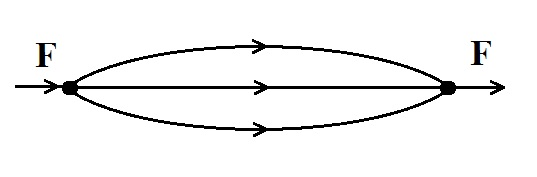
\includegraphics[width=0.60\linewidth]{img51.jpg}
	\caption{} \label{img:img5.1}
\end{figure}

Пусть величина $\displaystyle T =\sum_{i=1}^n t_i(f_i,c_i) f_i$ соответствует суммарному времени, которое потратит $F=f_1 + \dots + f_n$ автомобилей, чтобы преодолеть участок пути, изображенный на рисунке \ref{img:img5.1} (рисунок для случая $n=3$), где $c_i$ пропускная способность маршрута $i$, $f_i$ -- количество автомобилей, выбравших данный маршрут, а $t_i(f_i,c_i)$ -- среднее время движения по нему. 

Здесь правилу $y=R(x)$ соответствует решение задачи минимизации величины $T$ при известных пропускных способностях маршрутов. Ее можно представить в виде задачи поиска:
$$\min_{f} \sum_{i=1}^n\int_{0}^{f_i}t_i(u,c_i)du$$
при условиях:
\begin{equation*}
\begin{cases}
\displaystyle \sum_{i=1}^n f_i = F, \\[3ex]
\displaystyle f_i \geqslant 0,~i=\overline{1,n}\\
\end{cases}
\end{equation*}

Таким образом, при фиксированных пропускных способностях $c=(c_1,...,c_n)$ получаем конкретное оптимальное распределение автомобилей по маршрутам $f=f(c)$.

Соответственно, выбор стратегии первого игрока из соотношения $ \displaystyle H_1(x^*,y^*) = \max_x H_1(x,R(x))$ соответствует поиску оптимальных пропускных способностей:

$$\min_c \sum_{i=1}^n t_i(f_i,c_i)f_i$$
при условии
$$\sum_{i=1}^n c_i \leqslant C$$ 

Здесь $f=(f_1,...,f_n)$ выбирается по указанному выше правилу $f=f(c)$.
\chapter{Лекция 10}

[примеры про продажу электричества]


\begin{align*}
&\min\limits_f \sum \limits_{(i,j) \in A)} \int\limits_0^{f_{ij}} \Theta_{ij}(\tau) d \tau \\
&\sum \limits_{i \in \omega_j} f_{ij} - \sum\limits_{i\in u_j} f_{ji} = d_j & \omega_j \text{ -- вход в $j$ дугу}\\
&f_{ij} \geq 0 & u_j \text{ -- исход из $j$ дуги}
\end{align*}
лучше бы рассмотреть с нуля.
\chapter{Лекция 11}
\section{Двухуровневая оптимизация}
\begin{align*}
&T= \min  \limits_{c} \sum \limits_{i=1}^n t_i(f,c)f_i\\
&\sum \limits_{i=1}^n C_i \leqslant C\\
&\text {где}: \min \limits_{f} \sum \limits_{i=1}^n \int \limits_{0}^f t_i(u,c)du=Y(c)\\
&\sum \limits_{i=1}^n f_i=F\\
&f_i \geqslant 0, \: \forall i= \overline{1,n}\\
\end{align*}

1. Линейная функция задержки $ t_i(f_i,c_i)=a_i+c_i f_i,\text {но тогда} \sum \limits_{i=1}^n \dfrac{1}{c_i} \geqslant \dfrac{1}{c}; $
Выведем решение:
\begin{align*}
f_i=
\begin{cases}
\dfrac{\dfrac{1}{c_i} \left [F+\sum \limits_{s=1}^k \dfrac{a_s}{c_s}\right ]}{\sum \limits_{s=1}^n  \dfrac{1}{c_s}}-\dfrac{a_i}{c_i}, \: i \leqslant k\\
0, \: i>k
\end{cases}
\end{align*}
где $k$ определяется из условий: $\sum \limits_{i=1}^k \dfrac{a_k-a_i}{c_i} \leqslant F < \sum \limits_{i=1}^{k+1} \dfrac{a_{k+1}-a_i}{c_i} $
Пусть используются все $n$ маршрутов (для удобства). То есть $k=n$
%\begin{align*}
%&f_i= \dfrac{\dfrac{1}{c_i} \left [ F+ \sum \limits_{s=1}\dfrac{a_s}{c_s} \right ]}{\sum \limits_{s=1}^n\dfrac{1}%{c_s}}-\dfrac{a_i}{c_i}, \: i=\overline{1,n}\\
%&T=\dfrac{\sum \limits_{i=1}^n F+\sum \limits_{s=1}^n \dfrac{a_s}{c_s}}{\sum \limits_{s=1}^n \dfrac{1}{c_s}}\\
%\end{align*}

\begin{align*}
&\sum \limits_{i=1}^n c_i \leqslant c\\
&f_i=
\begin{cases}
\dfrac{c_i \left [F+\sum \limits_{s=1}^n a_s b_s \right ]}{\sum \limits_{s=1}^k c_s}-a_i c_i, if \: i \leqslant k\\
0, \: i>k
\end{cases}
\end{align*}


Теперь предположим, что у нас $ F $ в такой окрестности, что $ k = n $, тогда $ f_i=\dfrac{c_i \left [F+ \sum \limits_{s=1}^n a_s b_s\right ]}{\sum \limits_{s=1}^n c_s} -a_i c_i $. Отсюда получаем, что

\begin{align*}
&T=\dfrac{F+\sum \limits_{s=1}^n a_s c_s }{\sum \limits_{s=1}^n c_s} \sum \limits_{i=1}^n  c_i \left [ \dfrac{F+\sum \limits_{s=1}^n a_s c_s }{\sum \limits_{s=1}^n c_s} -a_i \right ] \rightarrow \min \limits_{c}\\
& \sum \limits_{i=1}^n c_i \leqslant c
\end{align*}

Теперь запишем общий вид.
\begin{align*}
&T=\dfrac{F+\sum \limits_{s=1}^n a_s c_s }{\sum \limits_{s=1}^k c_s} \sum \limits_{i=1}^k  c_i \left [ \dfrac{F+\sum \limits_{s=1}^k a_s c_s }{\sum \limits_{s=1}^k c_s} -a_i \right ] \rightarrow \min \limits_{c}\\
& a_1 \leqslant...\leqslant a_n; \\
\end{align*}
Выпишем условие для $k$: 
\begin{align*}
\sum \limits _{i=1}^k c_i(a_k-a_i) \leqslant F < \sum \limits_{i=1}^{k+1} c_i(a_{k+1}-a_i)
\end{align*}

Эвристический подход.
Алгоритм для решения последней задачи 
\begin{align*}
&1.  C^0=(C_1^0,...,C_n^0), \: C_i^0 \geqslant 0, \: \forall i=\overline{1,n} \\
&2.  f^0=arg \left [ \min \limits_{f} (\sum \limits_{i=1}^n  \int \limits_{0}^{f_i} |\sum \limits_{i=1}^n f_i=F, \: f_i \geqslant 0, \: i=\overline{1,n} \right ] \\
&3. T^0= \sum \limits_{i=1}^n t_i(f^0, c_i^0)f_i^0\\
&4. \text{Сравнение $T^0$ в популяции. Выбираем 10 лучших} \\
&5. \text{Новая популяция. Следовательно 100 штук образуют линейную комбинацию}\\
&\text{нулевой популяции.} \\
&6. \text{Нахожим $T^1$ и выбираем 10 наилучших, затем сравниваем в 10-ю лучшими из}\\
&\text{ $T^0$ и берем 10 лучших из лучших}
\end{align*}



\chapter{Рекомендуемая литература}
\begin{enumerate}
\item <<Новое индустриальное общество>>, Джон Кеннет Гэлбрейт
\end{enumerate}


\end{document}





